%% Modello computazionale
% descrivere il problema della computazione distribuita nel nostro contesto

% io parto da questa architettura che funziona così...
% ho un'architettura di riferimento con una macchina/mainframe centralizzata che definisce e distribuisce il
% carico di lavoro ed il calcolo; ho tanti client trasparenti/coerenti con i browser e poi gli utenti
% Immagine di come funziona


%Architettura:
% Modello statico->
% DEfinizione di cos'è uno User
% DEfinizione di cos'è un uTask
% DEfinizione di cos'è un Task generico

% Modello astratto->
%% TASK: dal punto di vista astratto è la definizione di un'operazione data driven
% su un modello di dati in ingresso e un modello di uscita, in cui posso caratterizzare
% cosa ci sta im mezzo in modo preciso con associato un codice di esecuzione.
%% Utente: è una persona con una macchina con certe caratteistiche e certe skill lui
%% uTask: istanziazione di un task con un particolare codice su una particolare macchina su dei dati

% TODO nell'immagine metto anche un dispositivo mobile e un utente con 2 device
\begin{figure}[htb]
	\centering
	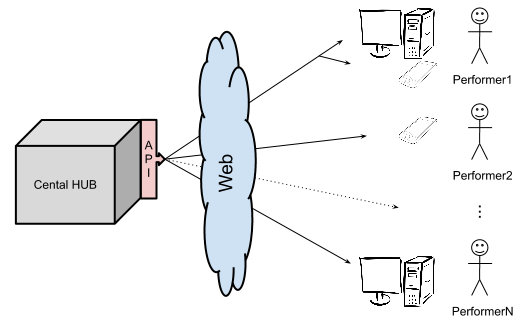
\includegraphics[width=0.75\columnwidth]{Architecture.png}
	\caption{Reference architecture.}
	\label{fig:architecture}
\end{figure}
The system use as a reference architecture the one depicted in \autoref{fig:architecture}.
Here we have a centralized hub that \emph{defines} and \emph{distribute} the workload,
a pletora of clients with their browsers and the users. The clients of this model
are all coherent and transparent to the execution of the code, wich is distributed
to the end-user according to the platform they are using.
As you can see the structure is almost the same as any other task distribution
platform, the strenghts of this system are in the characterization of the actors
in the system.

The reference model in \autoref{fig:architecture} has been customized to meet our
needs of flexibility and pluggability, so we introduced a \emph{configurator} and
a \emph{execution layer} in the central hub. These are the components that allow
our system to cover all the dimension presented in \autoref{tab:matrix}.

The \textbf{configurator} is in charge of defining and configuring a task in the
system, allowing the \emph{requester} to add hooks to exeternal resource in order
to manage the assignment cycle and the planning strategy.

The \textbf{execution layer} provides useful API for managing the \utask{} and
communicate with the \emph{configurator}.

\begin{figure}[tb]
	\centering
	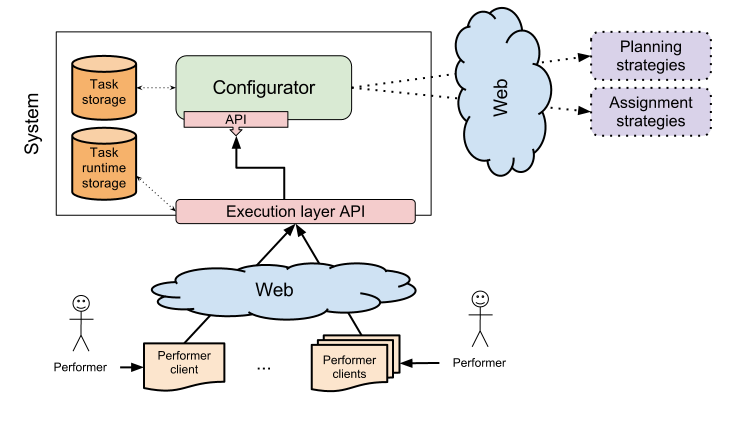
\includegraphics[width=\columnwidth]{Architecture2.png}
	\caption{Specialized architecture.}
	\label{fig:architecture2}
\end{figure}




% Subsection description

\subsection{Configurator}
\textbf{TODO}\\
This component is the kernel of the task creation and configuration. It is responsible
of the creation and the management of a \emph{Task}.

Provides
the following functionalities:
\begin{itemize}
	\item To allow a Requester to configure (at an abstract level) a new
	crowdsourced task by using the Configuration UI

	\item To allow a Task/Job Creator to monitor the execution of a crowdsourced
	task

	\item To allow a Performer to execute the assigned activity (Micro Task) by
	using a default, not configurable UI.

	\item To allow a CrowdSearcher Task/Job Client application to
	\begin{itemize}
		\item Create, configure, and monitor a (set of) Task(s), Please notice
		that the orchestration of several tasks is managed externally from
		CrowdSearcher.

		\item To retrieve the set of Micro Task associated with a Task.

		\item To post the result of a Micro Task execution.

		\item To get notified about the completion of a Task / MicroTask
	\end{itemize}
\end{itemize}

\subsection{Execution layer}
Execute
\subsection{Task sotrage \& task runtime storage}
Store
\subsection{Performer \& Performer client}
Performs
\subsection{Planning strategies}
Plan
\subsection{Assignment strategies}
Assign